\section{The Boltzmann Equation and the Lattice Boltzmann Method}\label{sec:collisionless boltzmann equation2}
The lattice Boltzmann method (LBM) is one of multiple widely-used computational approaches to model the behaviour of fluid flow with the aid of computers. It is based on the Boltzmann equation which can be written
\begin{equation}
  \frac{\partial f}{\partial t} + \mathbf{u}\cdot \nabla f = \Omega \left ( f \right ),
  \label{eq:boltzmann1}
\end{equation}
where $f(\mathbf{x},\mathbf{u},t)$ is the distribution function of the particle density $\rho$, over space $\mathbf{x}$, with velocity $\mathbf{u}$, at time $t$. Here, $\Omega$ represents the collision term. We furthermore assume that no external force is present.

Since the actual collision term is relatively expensive to implement, in practise typically the BGK collision term is used \cite{Bhatnagar1954}
\begin{equation}
    \Omega \left ( f \right ) = -\frac{1}{\tau} \left ( f - f^{eq}\right ),
\end{equation}
where $\tau$ is the relaxation time and $f^{eq}$ is the equilibrium function. 
 
The Boltzmann equation can be discretized in both time, physical and velocity space leading to the lattice Boltzmann method. In the lattice Boltzmann method a time step can be denoted as
\begin{equation}
    f_i \left ( \mathbf{x} +\mathbf{c}_i \delta t, t + \delta t \right ) = f_i \left (  \mathbf{x},t \right ) - \frac{\delta t}{\tau} \left ( f_i \left (  \mathbf{x},t \right ) - f_i^{eq}\left ( \mathbf{x} ,t \right ) \right ),
\end{equation}
where subscript $i$ denotes the velocity direction.

What sets the Boltzmann method apart from other CFD approaches is that a single time step can be split into two consecutive parts, the so-called streaming and collision steps. 

Writing the state of the system after collision as $f_i^\star \left (\mathbf{x}, t \right )$ we can get
\begin{equation}
f_i^\star \left (\mathbf{x},t \right ) = f_i \left ( \mathbf{x},t \right ) - \frac{\delta t}{\tau} \left ( f_i\left (\mathbf{x},t \right ) - f_i^{eq} \left ( \mathbf{x},t \right ) \right ),   
\end{equation}
for the collision step. Subsequently the streaming step is written as
\begin{equation}
    f_i \left ( \mathbf{x}+\mathbf{c}_i\delta t, t + \delta t \right ) = f_i^\star \left ( \mathbf{x},t \right ).
\end{equation}

This ability to split the equation into two separate physically motivated steps leads to the Boltzmann method being implemented by performing collision and streaming separately and consecutively. 

A popular way of classifying different combinations of dimensions and number of possible velocities is the so-called D$d$Q$q$ scheme. Here, $d$ denotes the number of space dimensions considered and $q$ the number of distinct velocities. In Figures \ref{fig:multiple_D1Qm} and \ref{fig:multiple_D2Qm}
 we give four examples of different combinations of D$d$Q$q$ possible.
In these lecture notes we are only considering the D1Q3, D2Q9 and D3Q27 cases. 
 \begin{figure}
     \centering
     \begin{minipage}{.48\textwidth}
         \centering
         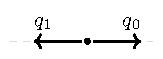
\includegraphics[width=\textwidth]{imgs/classical_cfd/D1Q2.pdf}
         \caption{D1Q2 lattice discretization.}
         \label{subfig:1aa}
     \end{minipage}
     \hfill
          \begin{minipage}{0.45\textwidth}
         \centering
         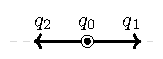
\includegraphics[width=\textwidth]{imgs/classical_cfd/D1Q3-2.pdf}
         \caption{D1Q3 lattice discretization.}
         \label{subfig:1ba}
     \end{minipage}
    \caption{Two examples of different types of D$d$Q$q$ possible for the 1-dimensional case. Figure \ref{subfig:1aa} portrays the D1Q2 setting and Figure \ref{subfig:1ba} portrays the D1Q3 setting (where a stationary particle can be included).}
     \label{fig:multiple_D1Qm}
\end{figure}

 \begin{figure}
     \centering
     \begin{minipage}{.48\textwidth}
         \centering
         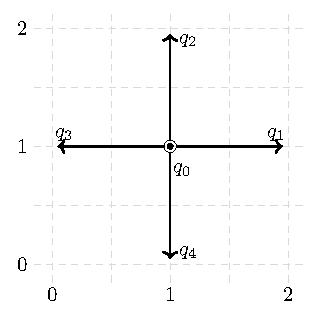
\includegraphics[width=\textwidth]{imgs/classical_cfd/D2Q5.pdf}
         \caption{D2Q5 lattice discretization.}
         \label{subfig:1a-2}
     \end{minipage}
     \hfill
          \begin{minipage}{0.45\textwidth}
         \centering
         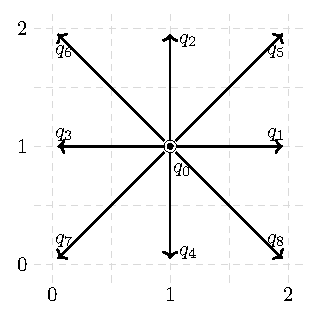
\includegraphics[width=\textwidth]{imgs/classical_cfd/D2Q9.pdf}
         \caption{D2Q9 lattice discretization.}
         \label{subfig:1b-2}
     \end{minipage}
    \caption{Two examples of different types of D$d$Q$q$ possible for the 2-dimensional case. Figure \ref{subfig:1a-2} portrays the D2Q5 setting and Figure \ref{subfig:1b-2} shows the D2Q9 setting. }
     \label{fig:multiple_D2Qm}
\end{figure}


We furthermore write $\mathbf{e}_i$ to represent the vector in the direction $i \in Q=\{0, 1, \dots,q-1\}$ of the D$d$Q$q$ scheme. For example, in the D2Q9 system we have
\begin{equation}
    \mathbf{e}_i = \begin{cases}
      (0,0) & \text{for $i = 0$}\\
      (1,0), (0,1), (-1,0), (0,-1) & \text{for $i = 1,2,3,4$}\\
      (1,1), (-1,1), (-1,-1), (1,-1) & \text{for $i=5,6,7,8$}.
    \end{cases}   
\end{equation}
Therefore $2$ qubits are necessary to represent the speed in each dimension, as the three options `positive', `negative' and `standing still' need to be encoded. 

\subsection{The collisionless Boltzmann equation}
Throughout these lecture notes, we consider the special case that no external forces are present, i.e., $\mathbf{F}=\mathbf{0}$. Moreover, in this section we neglect the collision of molecules to arrive at the collisionless Boltzmann equation
\begin{equation}
  \frac{\partial f}{\partial t} + \mathbf{u}\cdot \nabla f = 0.
  \label{eq:collisionless_boltzmann}
\end{equation}

We assume that the speeds are discrete, i.e., $u^{(i)}\in\mathcal{U}^{(i)}=\{u_1,\dots ,u_{N_{v_i}}\}$. For the scope of these lecture notes we only consider velocities $\mathbf{u}=(u^{(1)},u^{(2)},u^{(3)})$, for which the relative difference in speed in the different dimensions is bounded by
\begin{equation}
    c_\text{rel} = \max \frac{|u^{(i)}|}{|u^{(j)}|}\leq 1.
\end{equation}
As detailed in Section \ref{ssec:class_reflection} this is not a conceptual limitation of our approach, but helps us to keep the number of corner cases to be considered separately small, which also improves the readability of the material. %Moreover, we will drop the superscript $(i)$ wherever possible to improve readability and remark that all operations involving particle speeds are performed dimension by dimension.

As the main focus of this section is to discuss our quantum algorithm for the collisionless Boltzmann equation (CQBM) we will refrain from presenting the derivation of the macroscopic balance equations and just mention that the conservation laws for mass, momentum, and total energy can be derived from the Boltzmann equation \eqref{eq:boltzmann1} as detailed, for instance, in Chapter 2.5 of \cite{Kremer:2010}.

\subsection{Grid definition and obstacle placement}\label{ssec:grid}
In order to keep track of the temporal evolution of the distribution function $f(\mathbf{x},\mathbf{u},t)$, we first define a computational grid with equidistant grid spacing in all two or three spatial dimensions and assign densities to the volumes centered around the grid points. The grid is set up in a straightforward fashion, and grid points can be identified using the Cartesian coordinates system. Obstacles are subsequently placed in between grid points as depicted in Figure~\ref{fig:grid}.

\begin{figure}[h]
\centering
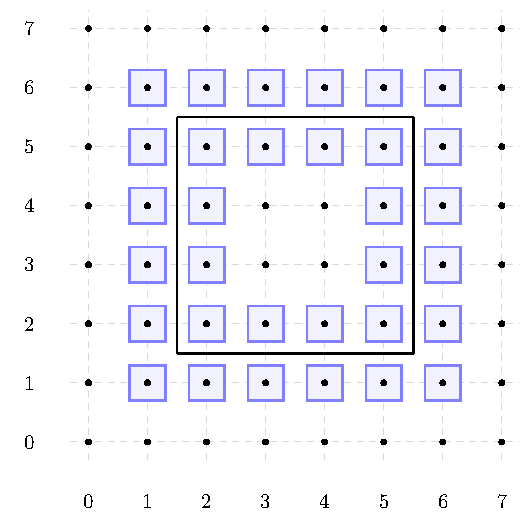
\includegraphics[]{imgs/classical_cfd/grid with obstacle.pdf}
%     \begin{tikzpicture}
%     \draw[help lines, color=gray!30, dashed] (-3.3,-3.3) grid (4.3,4.3);
%     \draw[thick,-,color=black] (-1.5,-1.5) -- (-1.5,2.5);
%     \draw[thick,-,color=black] (-1.5,-1.5) -- (2.5,-1.5);
%     \draw[thick,-,color=black] (2.5,-1.5) -- (2.5,2.5);
%     \draw[thick,color=black] (-1.5,2.5) -- (2.5,2.5);
    
%     \foreach \j in {0,...,3}
%     {
%         \node at (-1+\j,-1)[rectangle, draw=blue!50, fill=blue!5, thick, minimum size=0.6cm]{};
%         \node at (-1+\j,2)[rectangle, draw=blue!50, fill=blue!5, thick, minimum size=0.6cm]{};
%         \node at (-1,-1+\j)[rectangle, draw=blue!50, fill=blue!5, thick, minimum size=0.6cm]{};
%         \node at (2,-1+\j)[rectangle, draw=blue!50, fill=blue!5, thick, minimum size=0.6cm]{};
        
%     }
    
%     \foreach \j in {0,...,5}
%     {
%         \node at (-2+\j,-2)[rectangle, draw=blue!50, fill=blue!5, thick, minimum size=0.6cm]{};
%         \node at (-2+\j,3)[rectangle, draw=blue!50, fill=blue!5, thick, minimum size=0.6cm]{};
%         \node at (-2,-2+\j)[rectangle, draw=blue!50, fill=blue!5, thick, minimum size=0.6cm]{};
%         \node at (3,-2+\j)[rectangle, draw=blue!50, fill=blue!5, thick, minimum size=0.6cm]{};
        
%     }

%     \foreach \j in {0,...,7}
%     {
%         \foreach \i in {0,...,7} 
%         {
%             \node at (-3+\i,-3+\j)[circle, fill, color = black, inner sep=1pt]{};
%         }
%   }
   
%   \foreach \j in {0,...,7}
%   {
%         \node at (-4,-3+\j)[]{\j};
%         \node at (-3+\j,-4)[]{\j};
%   }



%     \end{tikzpicture}
    \caption{Illustration of an obstacle (black box) placed in a computational grid in two dimensions. The grid points (`$\cdot$' surrounded by blue boxes) surrounding the obstacle placement require special attention in our implementation. }
    \label{fig:grid}
\end{figure}

\subsection{Streaming}
In what follows we describe how to move the particles through space.
In the collisionless quantum Boltzmann method not all particles necessarily move in each time step. 
Furthermore, when a particle moves it does not necessarily move in all dimensions in the same time step. The velocity of each particle consists of a speed in each spatial dimension. Whether or not a particle will move in a given dimension depends on the speed in that dimension and whether or not a particle traveling at that speed will reach the next grid point in the current time step. 
This is due to the fact that we choose the size $\Delta t_m$ of time step $m$ to be such that some particles make it to the next grid point, but none overshoot. 
To make this idea more precise we define $u_\text{max} = \max_k |u_k|$ and $u_\text{min} = \min_k |u_k|$, with $u_k \in \mathcal{U} \coloneqq \bigcup_{i=1}^d \mathcal{U}^{(i)}$ the set of possible speeds a particle can travel. Then, we can normalize the distance between the grid points $\Delta x$ to enforce it will always be equal to $1$. Subsequently, the first time step $\Delta t_0$ will have size $\frac{1}{u_\text{max}}$. All particles that travel with speed $\pm u_{\text{max}}$ in a dimension will move one grid point in the first time step in that dimension. To determine the size $\Delta t_m$ of any subsequent time step $m$, we keep track of the distances a particle traveling at any of the possible speeds $u_k\in\mathcal{U}$ would be removed from reaching the next grid point and use this to find the smallest time step necessary for any particle to reach the next grid point in any dimension.

To ensure that particles can travel no further than the neighboring grid points, and thereby adhere to the CFL (Courant-Friedrichs-Lewy) condition, we use a so called CFL counter. This counter keeps track of the distances the particles are located from the next grid point based on their speed in each dimension and thereby determines the size of the next time step. 


\subsubsection{CFL counter}\label{ssec:cfl_counter}
In what follows, let $c^m_k$ represent how large of a fraction from the current grid point to the next a particle with speed $u_k$ has to travel.
We use the following expression
\begin{equation}
    c^{m+1}_{k} = c^m_{k} + |u_k| \frac{\Delta t_m}{\Delta x},
\end{equation}
where $u_k \in \mathcal{U}$ and $m$ represents the number of time steps that have been taken so far. Furthermore, $\Delta x$ represents the equidistant spacing between the grid points as before.  
It then follows that we can express the size of the time step taken in each iteration as
\begin{equation}\label{eq:delta_t}
    \Delta t_m = \min_{k} \left ( \left [1-c^m_{k} \right ] \frac{\Delta x}{|u_k|}  \right ).
\end{equation}
In the above equation we minimize over $k$ to ensure that at least one speed reaches the next grid point, and none overshoots. 

In a classical Boltzmann method $c_k^{m}$ can be used to interpolate the results when the simulation terminates in a time step that is not a complete cycle. This is not possible in the quantum counterpart and thus if we terminate the simulation in a time step that is not a complete cycle, some small oscillations will occur unless a post-smoothing method is applied. In this manuscript we restrict ourselves to running the CQBM algorithm for a total time $T = \sum_{m=0}^{N_t -1} \Delta t_m$ such that $\frac{T}{u_m} \in \mathbb{Z}$ $\forall m$. 

To complete the collisionless quantum Boltzmann method we need to describe the behavior when a particle collides with an obstacle. 

\subsection{Collision}
The collision step in the Boltzmann method is usually performed by taking a collision operator, such as the BGK operator \cite{Bhatnagar1954}, and performing a relaxation towards equilibrium. In these notes we will introduce the idea of equivalence classes, as used in the lattice gas models of the last century \cite{Yepez1998}. Two combinations of velocities belong to the same equivalence class if the resulting momentum is the same. Figure \ref{fig:equivalence_class} shows two combinations of velocities that belong to the same equivalence class for the D2Q5 case.

 \begin{figure}
     \centering
     \begin{minipage}{.48\textwidth}
         \centering
         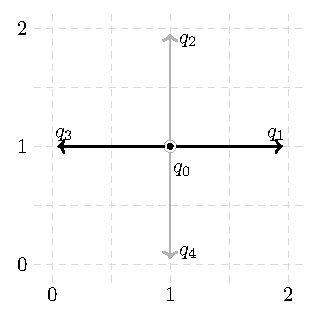
\includegraphics[width=\textwidth]{imgs/classical_cfd/equivalence_class_1.pdf}
         \caption{Equivalence class depiction for D2Q4 lattice discretization.}
         \label{subfig:1a}
     \end{minipage}
     \hfill
          \begin{minipage}{0.45\textwidth}
         \centering
         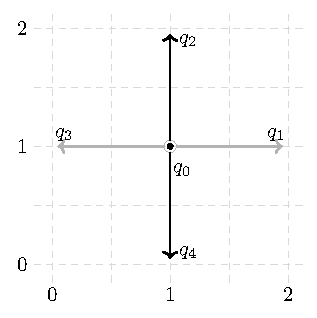
\includegraphics[width=\textwidth]{imgs/classical_cfd/equivalence_class_2.pdf}
         \caption{Equivalence class depiction for D2Q4 lattice discretization.}
         \label{subfig:1b}
     \end{minipage}
    \caption{Illustration of two velocity combinations of the D2Q5 (and D2Q4) velocity spectrum that belong to the same equivalence class with total momentum 0 and mass 2: (a) particles streaming in the $q_1$ and $q_3$ direction, and (b) particles streaming in the $q_2$ and $q_4$ direction. }
\label{fig:equivalence_class}
\end{figure}



\subsection{Reflection by an obstacle}\label{ssec:class_reflection}
In specular reflection, when a particle impinges on an object its velocity gets reflected along the axis normal to that object. 
Notice that due to this method we are restricted to modeling objects whose walls are either parallel or perpendicular to each dimension.
In order to facilitate the correct reflections we need to keep track of when a particle has come into contact with a wall, this is done differently for different values of $c_\text{rel}$.

We first consider the case $c_\text{rel} \leq 1$. In this case we know a particle has come into contact with an object if and only if it hits a grid point located in the first layer of the obstacle. We will refer to these grid points as the wall of the object. When a particle reaches a grid point in the wall of an object, its velocity normal to the wall gets reversed and the particle is moved one grid point outside of the object again in the direction normal to the wall(s) that just reflected it. Figure \ref{fig:specular reflection} gives an example of what such a reflection might look like.

\begin{figure}
\centering
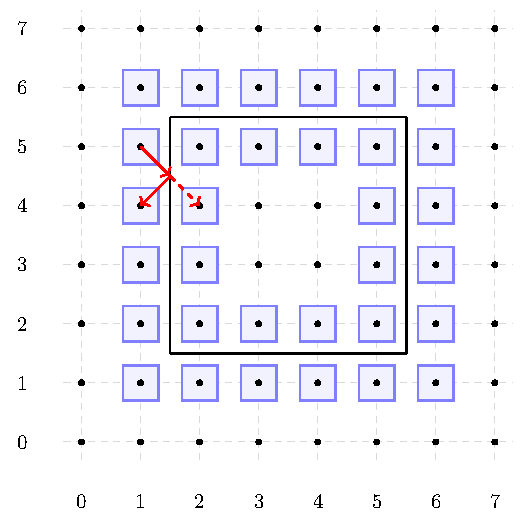
\includegraphics[]{imgs/classical_cfd/grid with reflection.pdf}
%     \begin{tikzpicture}
%     \draw[help lines, color=gray!30, dashed] (-3.3,-3.3) grid (4.3,4.3);
%     \draw[thick,color=black] (-1.5,-1.5) -- (-1.5,2.5);
%     \draw[thick,color=black] (-1.5,-1.5) -- (2.5,-1.5);
%     \draw[thick,color=black] (2.5,-1.5) -- (2.5,2.5);
%     \draw[thick,color=black] (-1.5,2.5) -- (2.5,2.5);
    
    
%     \foreach \j in {0,...,3}
%     {
%         \node at (-1+\j,-1)[rectangle, draw=blue!50, fill=blue!5, thick, minimum size=0.6cm]{};
%         \node at (-1+\j,2)[rectangle, draw=blue!50, fill=blue!5, thick, minimum size=0.6cm]{};
%         \node at (-1,-1+\j)[rectangle, draw=blue!50, fill=blue!5, thick, minimum size=0.6cm]{};
%         \node at (2,-1+\j)[rectangle, draw=blue!50, fill=blue!5, thick, minimum size=0.6cm]{};
        
%     }
    
%     \foreach \j in {0,...,5}
%     {
%         \node at (-2+\j,-2)[rectangle, draw=blue!50, fill=blue!5, thick, minimum size=0.6cm]{};
%         \node at (-2+\j,3)[rectangle, draw=blue!50, fill=blue!5, thick, minimum size=0.6cm]{};
%         \node at (-2,-2+\j)[rectangle, draw=blue!50, fill=blue!5, thick, minimum size=0.6cm]{};
%         \node at (3,-2+\j)[rectangle, draw=blue!50, fill=blue!5, thick, minimum size=0.6cm]{};
        
%     }
    
    
%     \foreach \j in {0,...,7}
%     {
%         \foreach \i in {0,...,7} 
%         {
%             \node at (-3+\i,-3+\j)[circle, fill, color = black, inner sep=1pt]{};
%             \node at (-3+\i,-3+\j)[circle, fill, color = black, inner sep=1pt]{};
%         }
%   }
%     \draw[->,color=red, thick] (-2,2) -- (-1.5,1.5);
%     \draw[->,dashed,color=red, thick] (-1.5,1.5) -- (-1,1) ;
%     %\draw[->,dashed,color=red, thick] (-1,1) -- (-1.5,0.5) ;
%     \draw[->,color=red, thick] (-1.5,1.5) -- (-2,1);
%     %\draw[->,dashed,color=red, thick] (-2,1) -- (-2.5,0.5) ;
    
%   \foreach \j in {0,...,7}
%   {
%         \node at (-4,-3+\j)[]{\j};
%         \node at (-3+\j,-4)[]{\j};
%   }

%     \end{tikzpicture}
    \caption{Illustration of an obstacle (black box) in the grid with the red arrow representing one possible collision operation. The dashed arrow represents the trajectory had no reflection taken place. }
    \label{fig:specular reflection}
\end{figure}

For $c_\text{rel} > 1$ the specular reflection step becomes more complicated, as grid points located outside the object can be reached by a particle indicating that the particle has come into contact with an object; See Figure \ref{fig:specular reflection c3}. Similarly multiple cases need to be taken into account to determine whether a particle hits a corner point of an object or the wall at a non-corner point. For simplicity we will restrict ourselves to the case $c_\text{rel} \leq 1$ for the scope of this paper, but we would like to remark that our method can be generalized to any value of $c_\text{rel}$ at the cost of taking into account more corner cases.

\begin{figure}
\centering
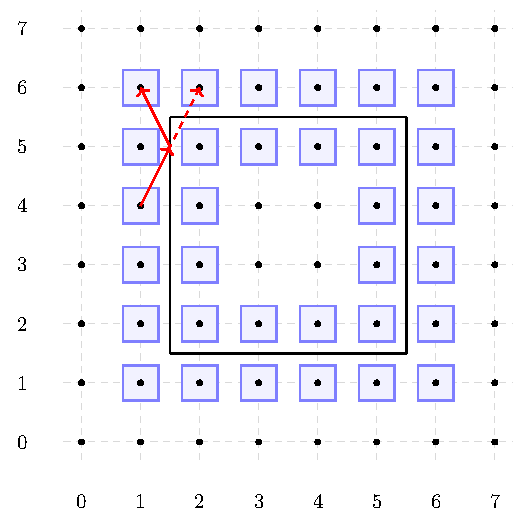
\includegraphics[]{imgs/classical_cfd/grid with reflection crel.pdf}
%     \begin{tikzpicture}
%     \draw[help lines, color=gray!30, dashed] (-3.3,-3.3) grid (4.3,4.3);
%     \draw[thick,color=black] (-1.5,-1.5) -- (-1.5,2.5);
%     \draw[thick,color=black] (-1.5,-1.5) -- (2.5,-1.5);
%     \draw[thick,color=black] (2.5,-1.5) -- (2.5,2.5);
%     \draw[thick,color=black] (-1.5,2.5) -- (2.5,2.5);
    
    
%     \foreach \j in {0,...,3}
%     {
%         \node at (-1+\j,-1)[rectangle, draw=blue!50, fill=blue!5, thick, minimum size=0.6cm]{};
%         \node at (-1+\j,2)[rectangle, draw=blue!50, fill=blue!5, thick, minimum size=0.6cm]{};
%         \node at (-1,-1+\j)[rectangle, draw=blue!50, fill=blue!5, thick, minimum size=0.6cm]{};
%         \node at (2,-1+\j)[rectangle, draw=blue!50, fill=blue!5, thick, minimum size=0.6cm]{};
        
%     }
    
%     \foreach \j in {0,...,5}
%     {
%         \node at (-2+\j,-2)[rectangle, draw=blue!50, fill=blue!5, thick, minimum size=0.6cm]{};
%         \node at (-2+\j,3)[rectangle, draw=blue!50, fill=blue!5, thick, minimum size=0.6cm]{};
%         \node at (-2,-2+\j)[rectangle, draw=blue!50, fill=blue!5, thick, minimum size=0.6cm]{};
%         \node at (3,-2+\j)[rectangle, draw=blue!50, fill=blue!5, thick, minimum size=0.6cm]{};
        
%     }
    
%     % \foreach \j in {0,1}
%     % {
%     %     \foreach \i in {0,1}
%     %     {
%     %     \node at (-3+2 + 3*\j,-2+5*\i)[rectangle, draw=green!50, fill=blue!5, thick, minimum size=0.6cm]{};
%     %     \node at (-2+5*\i,-3+2 + 3*\j)[rectangle, draw=orange!50, fill=blue!5, thick, minimum size=0.6cm]{};
%     %     }
%     % }
    
%     \foreach \j in {0,...,7}
%     {
%         \foreach \i in {0,...,7} 
%         {
%             \node at (-3+\i,-3+\j)[circle, fill, color = black, inner sep=1pt]{};
%             \node at (-3+\i,-3+\j)[circle, fill, color = black, inner sep=1pt]{};
%         }
%   }
%     \draw[->,color=red, thick] (-1.5,2) -- (-2,3) ;
%     \draw[->,color=red, thick] (-2,1) -- (-1.5,2) ;
%     \draw[->,dashed,color=red, thick] (-2,1) -- (-1,3) ;
    
%   \foreach \j in {0,...,7}
%   {
%         \node at (-4,-3+\j)[]{\j};
%         \node at (-3+\j,-4)[]{\j};
%   }

%     \end{tikzpicture}
    \caption{Illustration of an obstacle (black box) in the grid with the red arrow representing one possible specular reflection operation when $c_\text{rel} > 1$ holds. The dashed arrow represents the trajectory had no reflection taken place. }
    \label{fig:specular reflection c3}
\end{figure}

\section{Momentum Exchange Method}\label{sec:MEM}
The momentum exchange method was proposed by Ladd \cite{Ladd1994} to determine the force acting on an object in order to calculate the drag and lift coefficients of an obstacle equipped with bounce back boundary conditions when the flow field is modelled by the Boltzmann method. Bounce back boundary conditions differ from the more intuitive specular reflection boundary conditions in that, upon contact with an object, the particle's velocity is reversed entirely instead of just the velocity normal to the object; see Figure \ref{fig:bounce_back_vs_specular_reflection}. Bounce back boundary conditions are often used in combination with the Lattice Boltzmann method \cite{Kruger2017}. In Section \ref{sec:qbb} we give an in-depth explanation of bounce back boundary conditions as well as how to implement them in our QLBM scheme.
In this paper we adopt the momentum exchange method as described in \cite{Kruger2017}. Then the force exerted on the object by the particles can be expressed as
\begin{equation}\label{eq:F1}
    \mathbf{F} = \sum_{i\in Q} \left ( \mathbf{e}_{i}f_i(\mathbf{x}_f,t) - \mathbf{e}_{\bar{i}} f_{\bar{i}}(\mathbf{x}_f,t) \right ) .
\end{equation}
In the above expression $\mathbf{x}_f$ refers to a point in the fluid space adjacent to the obstacle and $\bar{i}$ represents the velocity of the particles after particles with velocity $i$ have impinged on the object.
$Q$ is the set of all distinct velocities in the discretization.
This expression assumes that there is no fluid inside the object and as such only takes the momentum exchange outside of the object into account. Since we are using bounce back boundary conditions we have $\mathbf{e}_{\bar{i}}:=-\mathbf{e}_i$ and
$f_i(\mathbf{x}_f,t) = f_{\bar{i}}(\mathbf{x}_f,t)$ by definition, therefore we can rewrite Equation \eqref{eq:F1} to 
\begin{equation}\label{eq:F2}
    \mathbf{F} = \sum_{i\in Q} 2 \mathbf{e}_{i} f_i(\mathbf{x}_f,t).
\end{equation}
As force is composed of magnitude and direction it is expressed by a $d$ dimensional vector with subscript $j$ denoting its $j$-th dimensional component, i.e.
\begin{equation}\label{eq:F2_d}
    F_j = \left ( \sum_{i\in Q} 2 \mathbf{e}_{i} f_i(\mathbf{x}_f,t) \right )_j.
\end{equation}